%%%%%%%%%%%%%%%%%%%%%%%%%%%%%%%%%%%%%%%%%%%%%%%%%%%%%%%%%%%%%%%%%%%%%%%%%%%
%
% Plantilla para un artículo en LaTeX en español.
%
%%%%%%%%%%%%%%%%%%%%%%%%%%%%%%%%%%%%%%%%%%%%%%%%%%%%%%%%%%%%%%%%%%%%%%%%%%%

% Qué tipo de documento estamos por comenzar:
\documentclass[a4paper]{article}
% Esto es para que el LaTeX sepa que el texto está en español:
\usepackage[spanish]{babel}
\selectlanguage{spanish}
% Esto es para poder escribir acentos directamente:
\usepackage[utf8]{inputenc}
\usepackage[T1]{fontenc}



%% Asigna un tamaño a la hoja y los márgenes
\usepackage[a4paper,top=3cm,bottom=2cm,left=3cm,right=3cm,marginparwidth=1.75cm]{geometry}

%% Paquetes de la AMS
\usepackage{amsmath, amsthm, amsfonts}
%% Para añadir archivo∫s con extensión pdf, jpg, png or tif
\usepackage{graphicx}
\usepackage[colorinlistoftodos]{todonotes}
\usepackage[colorlinks=true, allcolors=blue]{hyperref}

%% Para dar tamaño a las celdas de las tablas
\usepackage{array}
\newcolumntype{C}[1]{>{\centering\let\newline\\\arraybackslash\hspace{0pt}}m{#1}}


%% Primero escribimos el título
\title{Problema de la Satisfacibilidad Booleana}
\author{Fernanda Domínguez Acosta, Ximena Sandoval del Hoyo, Raúl Murcia Yocupicio}


%% Después de "preámbulo", podemos empezar el documento

\begin{document}
%% Hay que decirle que incluya el título en el documento
\maketitle

%% Iniciamos "secciones" que servirán como subtítulos

\section{Definiciones}

\subsection{Verificador}
Para cierto tipo de problemas evadir búsquedas de fuerza bruta para encontrar
soluciones a ellos no ha sido posible, por tanto no se conocen algoritmos para
resolver dichos problemas en tiempo polinomial.
Para estos problemas si bien no tenemos una forma rápida (i.e. en tiempo
polinomial), si encontraramos una solución de alguna manera (usando un algoritmo
de tiempo exponencial), podemos verificar facilmente dicha solución.
Es decir, verificar la solución es más facil que determinar su existencia.

Un verificador para un lenguaje $A$ es un algoritmo $V$, donde
\begin{center}
$A = \{w$ | $V$ acepta $\langle w, c\rangle$ para alguna cadena $c\}$
\end{center}
Determinamos el tiempo de un verificador solo en terminos de $w$, por lo que un
\textbf{verificador en tiempo polinomial} corre en un tiempo polinomial sobre la
longitud de $w$. Un lenguaje $A$ es polinomialmente verificable si tiene un
verificador en tiempo polinomial.
Este verificador utiliza información adicional almancenada en $c$ para verificar
si $w \in A$; esta información se llama \textbf{certificado} o \textbf{prueba}.

\subsection{Definición de Problema NP}

Sea $L$ un lenguaje (un problema). Decimos que $L$ pertenece a la clase
$\mathcal{NP} \Leftrightarrow \exists$ una MT \textbf{no determinista} $M$
tal que $L = L(M)$ y $T_M(n)$ (Time-Complexity de $M$) sea un polinomio.

Alternativamente, $L \in \mathcal{NP} \Leftrightarrow$ $L$ tiene verificadores
en tiempo polinomial.


%aaaaaaaaaaaaaaaaaaaaaaaaaaaaaaaaa
%aaaaaaaaaaaaaaaaaaaaaaaaaaaaaaaaa
%aaaaaaaaaaaaaaaaaaaaaaaaaaaaaaaaa
%aaaaaaaaaaaaaaaaaaaaaaaaaaaaaaaaa
%aaaaaaaaaaaaaaaaaaaaaaaaaaaaaaaaa
%aaaaaaaaaaaaaaaaaaaaaaaaaaaaaaaaa
%aaaaaaaaaaaaaaaaaaaaaaaaaaaaaaaaa


\subsection{Reducciones polinómicas}
Nuestra principal metodología para probar que un problema $P_2 \notin \mathcal{P}$
es la reducción de un problema $P_1$, sabiendo que $P_1 \notin \mathcal{P}$, a $P_2$.

\begin{figure}[h]
\centering
\graphicspath{ {./Images/} }
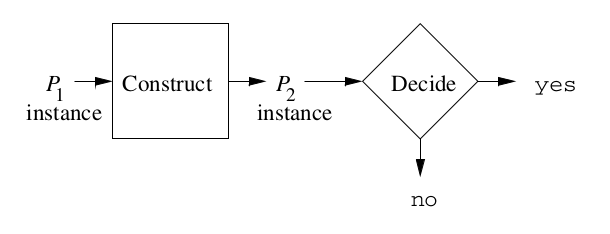
\includegraphics[width=0.5\textwidth]{reduccion.png}
\caption{\label{fig:Reduccion}Esquema de reducción\cite{hopcroft2001introduction}}
\end{figure}
Sin embargo, la existencia de un algoritmo llamado ``Construct'' no es suficiente
para probar ``Si $P_1$ no está en $\mathcal{P}$ entonces $P_2$ tampoco está en $\mathcal{P}$''.

Supongams que dada una instancia de $P_1$ de longitud $m$, podemos encontrarnos
con dos situaciones:
\begin{itemize}
  \item El algoritmo de construcción produce una cadena de salida con longitud
  $2^{m}$, que entra en el hipotético algoritmo polinomial de $P_2$. Si este
  algoritmo toma un tiempo $\mathcal{O}(n^k)$ entonces con una cadena de
  longitud $2^{m}$ tomará un tiempo $\mathcal{O}(2^{km})$, exponencial sobre $m$.
  \item El algoritmo de construcción produce una cadena de salida con longitud
  $m$ pero toma un tiempo exponencial en ello, como $\mathcal{O}(2^m)$. Ahora el
  algoritmo de decisión para $P_2$ toma un tiempo polinomial $\mathcal{O}(n^k)$
  para una entrada de tamaño $n$ pero el algoritmo de decisión para $P_1$ toma
  $\mathcal{O}(2^{m} + m^{k})$.
\end{itemize}
Estos hechos implican que $P_1 \notin \mathcal{P}$ y $P_2 \in \mathcal{P}$

La restricción correcta para una construcción de $P_1$ a $P_2$ es que  ésta requiere
un tiempo polinomial sobre el tamaño de la entrada.
Esto implica que dicha construcción toma un tiempo $\mathcal{O}(m^{j})$ es un
cadena de longitud $m$, por lo que la instancia de $P_2$ no puede ser mayor al
número de pasos que tomó, es decir, a lo más $cm^{j}$ para una constante $c$.
Con esto podemos probar que si $P_2 \in \mathcal{P}$ entonces $P_1 \in \mathcal{P}$.

Supongamos que podemos decidir si una cadena de longitud $n$ pertenece a $P_2$
en un tiempo $\mathcal{O}(n^{k})$. Entonces podemos probar si una cadena de
longitud $m$ pertenece a $P_1$ en $\mathcal{O}(m^j + (cm^j)^k)$,
donde $m^j$ corresponde al tiempo del algoritmo de construcción y $(cm^j)^k$ al
tiempo para decidir si el resultado de la construcción pertenece a $P_2$.
Notamos que al simplificar el tiempo para $P_1$ obtenemos
$\mathcal{O}(m^j + (cm^{jk})$, donde $c$, $j$ y $k$ son constantes, por lo que
el tiempo es polinomial sobre $m$, por lo que podemos concluir que $P_1 \in \mathcal{P}$.

\subsection{Definición de Problema NP-Completo}
Sea $L$ un lenguaje (un problema). Decimos que $L$ es $NP-completo$ si las
siguientes afirmaciones son correctas sobre $L$:
\begin{enumerate}
  \item $L \in \mathcal{NP}$
  \item Para todo $L' \in \mathcal{NP}$, existe una reducción polinómica de $L'$ a $L$
\end{enumerate}

%AAAAAAAAAAAAAAAAAAAAAAAAAAAAAAA

\section{El problema de satisfacibilidad}
%Descripción
El problema de la satisfacibilidad booleana es un problema NP-completo\cite{cook1971complexity}.



\subsection{Codificación del problema}

Las variables se identifican con

\section{Demostración}
Para demostrar que SAT es NP-Completo, primero tenemos que demostrar que es de la clase NP.

\subsection{SAT pertenece a la clase NP}
así es

\subsection{SAT pertenece a la clase NP-Completo}
Ahora para demostrar que el SAT pertenece a la clase NP-Completo, debemos demostrar que todo problema en la clase $\mathcal{NP}$ se puede reducir al SAT en un tiempo polinomial. Esto es, necesitamos encontrar un algoritmo que, dada una instancia $w$ de un problema $L \in \mathcal{NP}$, nos devuelva una fórmula en lógica de orden cero (una instancia del SAT) tal que esta sea satisfacible si y sólo si $w\in L$\\

%. Nótese que este algoritmo se generaliza para toda NTM (Non-deterministic Turing %Machine) $M$, por lo que si se fija para una sola $M$, el resultado de este sólo %dependerá de $w$.

Sea $L \in \mathcal{NP}$. Por definición, existe una NTM (Non-deterministic Turing Machine) $M$ que acepta a $L$ como lenguaje. Sea $w$ una instancia de $L$, de forma que la entrada del algoritmo será $<M,w>$. Podemos asumir que la NTM $M$ no realiza mas de $p(n)$ pasos sobre la cadena $w$ de longitud $n$ en cualquier rama, donde $p(n)$ es un polinomio (por definición de la clase $\mathcal{NP}$). Esto significa que podemos asumir que el tamaño de la cinta utilizado será de a lo más, $p(n)$ celdas. También podemos asumir que $M$ nunca escribe el símbolo $\sqcup$, y nunca mueve el cabezal hacia la izquierda de su posición inicial (Máquina de Turing con cinta semi-infinita).
Partiendo de esto, es posible representar una descripción instantánea (en este caso la configuración inicial) de la máquina de la siguiente manera.

\begin{table}
  \begin{center}
    \begin{tabular}{| c | c | c | C{2cm} | c | c | C{4cm} | c |}
      \hline
      $q_0$ & $w_1$ & $w_2$ & $\dots$ & $w_n$ & $\sqcup$ & $\dots$ & $\sqcup$\\
      \hline
      %$w_1$ & $p$ & $w_2$ & $\dots$ & $w_n$ & $\sqcup$ & $\dots$ & $\sqcup$\\
      %\hline
      %\multicolumn{8}{|c|}{$\cdots$}\\
      %\hline
      %$f$ & $w_1$ & $w_2$ & $\dots$ & $w_n$ & $\sqcup$ & $\dots$ & $\sqcup$\\
      %\hline
    \end{tabular}
  \end{center}
\end{table}

De esta forma, un historial de cómputo (o una rama de cómputo de la NTM) se puede representar como una tabla cuyos renglones son las descripciones instantáneas en cada paso.\\
\begin{table}[h]
  \begin{center}
    \begin{tabular}{| c | c | c | C{2cm} | c | c | C{4cm} | c |}
      \hline
      $q_0$ & $w_1$ & $w_2$ & $\dots$ & $w_n$ & $\sqcup$ & $\dots$ & $\sqcup$\\
      \hline
      $w_1$ & $p$ & $w_2$ & $\dots$ & $w_n$ & $\sqcup$ & $\dots$ & $\sqcup$\\
      \hline
      \multicolumn{8}{|c|}{$\cdots$}\\
      \hline
      $f$ & $w_1$ & $w_2$ & $\dots$ & $w_n$ & $\sqcup$ & $\dots$ & $\sqcup$\\
      \hline
    \end{tabular}
  \end{center}
\end{table}

Una tabla con un historial de cómputo válido que llega a un estado de aceptación existe, si y sólo si, la cadena $w$ es aceptada por $M$. Por lo tanto buscaremos una fórmula que nos permita determinar si existe dicho historial de cómputo.\\
Consideremos la siguiente notación para describir a la tabla.
$$X_{i,j,\alpha} = \text{TRUE} \iff X_{i,j} = \alpha$$
donde $X_{i,j}$ es el contenido de la casilla de la tabla, en el renglón $i$ y columna $j$, y el símbolo $\alpha \in Q\cup\Gamma$, donde $Q$ es el conjunto de estados y $\Gamma$ es el alfabeto de cinta de $M$.\\

Cuatro restricciones deben cumplirse para determinar si dicho historial existe.

\begin{itemize}
  \item 1. Cada celda tiene un símbolo único ($\Phi_{\text{CELL}}$).
  \item 2. El primer renglón representa la configuración inicial de $M$ ($\Phi_{\text{START}}$).
  \item 3. Aparece un estado de aceptación en alguna casilla ($\Phi_{\text{ACCEPT}}$).
  \item 4. Todo movimiento en la tabla es legal ($\Phi_{\text{MOVE}}$).
\end{itemize}

De forma que si se cumplen estas cuatro restricciones, significa que $M$ acepta a $w$, por lo tanto debemos encontrar una fórmula que represente estas cuatro restricciones.
Se propone la siguiente:
$$\Phi = \Phi_{\text{CELL}} \land \Phi_{\text{START}} \land \Phi_{\text{ACCEPT}} \land \Phi_{\text{MOVE}}$$
Se describirá la construcción de cada una de ellas.

\paragraph{Restricción 1. $\Phi_{\text{CELL}}$.}

Para esta restricción simplemente debemos tener un OR exclusivo entre los $X_{i,j,\alpha}$ $\forall \alpha \in Q \cup \Gamma$ con $i$, $j$ fijos. Esto es:
\begin{align*}
  \Phi_{\text{CELL}} = \bigvee_{i,j} \Big[ &(X_{i,j,\alpha_1} \land \overline{X_{i,j,\alpha_2}} \land \dots \land \overline{X_{i,j,\alpha_k}}) \\
  &(\overline{X_{i,j,\alpha_1}} \land X_{i,j,\alpha_2} \land \dots \land \overline{X_{i,j,\alpha_k}})\\
  &\vdots\\
  &\overline{(X_{i,j,\alpha_1}} \land \overline{X_{i,j,\alpha_2}} \land \dots \land X_{i,j,\alpha_k}) \Big]
\end{align*}
El tamaño de este término es del orden de $p(n)^2$, pues $k$ es una constante que depende de $M$.

\paragraph{Restricción 2. $\Phi_{\text{START}}$.}

Para la siguiente restricción es necesario verificar que en el primer renglón se encuentre la configuración inicial. Esto es:
$$\Phi_{\text{START}} = X_{1,1,q_0} \land X_{1,2,w_1} \land X_{1,3,w_2} \land \dots \land X_{1,n+1,w_n} \land X_{1,n+2,\sqcup} \land X_{1,n+3,\sqcup} \land \dots \land X_{1,p(n)+1,\sqcup}$$
donde $w_i$ es el i-ésimo símbolo de la cadena $w$. Este término depende de $w$, pero siempre tendrá longitud de $p(n)$.

\paragraph{Restricción 3. $\Phi_{\text{ACCEPT}}$.}

Esta restricción solo tiene que asegurarse que en algún punto se llegue al estado de aceptación, pues podemos suponer que el estado de aceptación es único y que además, marca una parada en la NTM.
$$\Phi_{\text{ACCEPT}} = \bigvee_{i, j} X_{i,j,p}$$
donde p es el estado de aceptación. Esta restricción solo depende de $M$, y tiene tamaño del orden de $p(n)^2$.


\paragraph{Restricción 4. $\Phi_{\text{MOVE}}$}

Esta última restricción se logra con una conjunción de $\Omega_i$ con $i = 1,2,\dots,p(n)$, donde cada $\Omega_i$ significa que la descripción instantánea del renglón $i+1$ puede proceder correctamente a la del renglón $i$. Esto se logra asegurando dos cosas en cada $\Omega_i$.

\begin{itemize}
  \item $\xi_{i,j}$ significa:
    \begin{itemize}
      \item \textbf{a)} $X_{i,j} \not \in Q$ ($i.e$ $X_{i,j}$ no es un estado).
      \item \textbf{b)} Si no hay un estado adyacente a $X_{i,j}$ ($i.e.$ ni $X_{i,j-1}$ ni $X_{i,j+1}$ son estados), entonces $X_{i,j}=X_{i+1,j}$.
    \end{itemize}
  \item $\psi_{i,j}$ significa:
    \begin{itemize}
      \item \textbf{a)} $X_{i,j} \in Q$ ($i.e$ $X_{i,j}$ es un estado).
      \item \textbf{b)} Existe un posible movimiento de $M$ tal que $X_{i,j}$ es el estado y $X_{i,j+1}$ es el símbolo escaneado, de forma que $X_{i,j-1} X_{i,j} X_{i,j+1}$ se transforma en $X_{i+1,j-1} X_{i+1,j} X_{i+1,j+1}$. Es importante mencionar que si $X_{i,j}$ es un estado de aceptación, entonces existe la opción de no realizar movimiento, de forma que las siguientes descripciones instantáneas serán iguales.
    \end{itemize}
\end{itemize}
De esta forma tenemos que:
$$\Omega_i = \bigwedge_{j=1}^{p(n)}\left(\xi_{i,j}\land\psi_{i,j}\right)$$


% Ejemplo de figurita que puede ayudar después
%\begin{figure}
%\centering
%\includegraphics[width=0.5\textwidth]{tesla.jpg}
%\caption{\label{fig:tesla}Esta imagen se añadió en el menú Project.}
%\end{figure}


\bibliographystyle{plain}
\nocite{*}
\bibliography{main}

% Nota
%Para las bibliografías está rotísimo, para que salga todo hay que hacer:
% pdflatex main.tex -f
% bibtex main
% pdflatex main.tex -f
% pdflatex main.tex -f
%
% Dos veces al final

\end{document}
